\documentclass[12pt]{article}
\usepackage{graphicx} %required for inserting images
\graphicspath{{./images/}}
\usepackage{array}
\usepackage{lipsum}
\usepackage{comment}
\usepackage{amsmath}
%flowchart drawing package




%Tiles making sections
\title{GEOTECHNICAL DESIGN OF DRIVEN PILES UNDER AXIAL LOADS}
\author{Sakib Bin Rafi Tonmoy,Jakaria Pervez}
\date{05/04/2023}
%End for tiltles
\begin{document}
\maketitle

%%Begining of Introduction
\section{Settlement of Piled-Raft System with floating piles }
 If concrete columns are not end bearing, the settlement may become an issue. The settlement of concrete column-reinforced soft foundations can be estimated using the method for piled rafts or pile groups.Horikoshi and Randolph (1999) and Poulos (2001) proposed simplified design methods to calculate the settlement of piled rafts, which are based on pile–raft interaction. \\
 
 
 %%adding figure for equivalent pier
\begin{figure}[h]
\centering
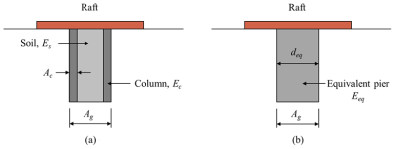
\includegraphics{Equivalent_Pier}
\caption{Equivalent Pier}
\label{fig:eqv_pier}
\end{figure}

%%end of figure


Randolph (1999) used the equivalent pier concept for the piled raft method as shown in \ref{fig:eqv_pier}.Independent parameters that are required known before calculation are as follows:
%%parameters for settlement calcualtion
\begin{equation*}
\begin{align*}
&\text{Material Properties}:\\
E_c&=\text{modulus of Elasticity for pile materials in Mpa}\\
E_s&=\text{modulus of Elasticity for soil in Mpa}\\
\nu &=\text{Poisson's ratio for soil}\\
G_L&=\text{shear modulus of the soil at the base of columns MPa}\\
G_b&=\text{shear modulus of the soil below the base of columns Mpa}\\
G_{avg}&=\text{average shear modulus of the soil within the length of columns Mpa}\\\\
&\text{column Properties}:\\
N_{cl}&=\text{Number of columns}\\
s&=\text{spacings of column in meter}\\
L_c&=\tect{Length of column in meter}\\
r_c&=\text{radius of pile}\\
A_{ci}&=\text{Area of ith column in meter}\\\\
&\text{Raft Properties}\\
L_r&=\text{Length or Diameter of the raft}\\
B_r&=\text{Width or Diameter of the raft}\\
I_s&=\text{Influence Factor 0.88 for square raft or 0.79 for circular raft}\\
\end{align*}
\end{equation*}
%%End of Introduction of Introduction

\section{Calcualtion Steps}
\noindent \text{Step1:Calcualte Shear Modulus of Soil}\\
\begin{equation*}
\begin{align*}
G_L&=\text{shear modulus of the soil at the base of columns MPa}\\
G_b&=\text{shear modulus of the soil below the base of columns Mpa}\\
G&=\frac{E}{2(1+\nu)}\\
G_{avg}&=\frac{G_L+G_b}{2}\\
\zeta&=\frac{G_L}{G_b}\\
\rho&=\frac{G_{avg}}{G_L}
\end{align*}
\end{equation*}







%\lipsum[2]
%writing necessary equation



\begin{comment}

\begin{center}
\begin{table}
\begin{tabular}{|m{10cm}|m{2cm}|m{4cm}|}
\hline

                   & Limiting f,kips/fit^2(kPa) \\
\hline
Very loose & 15 & 1.0 (47.8)\\
\hline
Loose & 20 & 1.4 (67.0)\\
\hline
Medium & 25 & 1.7 (83.1)\\
\hline
Dense & 30 & 2.0 (95.5)\\
\hline
\end{tabular}
\caption{\label{f_non_cohesive}uideline for Side Friction in Siliceous Soil}
\end{table}

\end{center}

\end{comment}
\end{document}